% !TEX root = ../main.tex
\chapter{Розрахунок періодів квантування}
\section{Розрахунок на умові забезпечення необхідної точності керування}
За цим критерієм період квантування обчислюється з умови $T_0 \leq \frac{\varepsilon}{B_{\max}}$,
де $B_{\max}$ -- максимальне значення функції $B(\omega) = \omega A(\omega)$, а $A(\omega)$ --
амплітудно-частотна характеристика (АЧХ) об'єкта.
$B(\omega)$ описує верхню границю можливих швидкостей зміни сигналу на виході об'єкта.
\subsection{Випадок \texorpdfstring{$W_{O_1}(s) = \frac{k e^{-\tau s}}{T_1 s + 1}$}{1}}
Знайдемо $B(\omega)$:
\begin{gather}
    B(\omega) = \omega A(\omega) = \omega \cdot \left| W_{O_1}(j \omega)\right| = 
    \omega \cdot \frac{
        k \left| e^{-\tau j \omega}\right|
    }{
        \left|T_1 j \omega + 1\right|
    } = \frac{k \omega}{\sqrt{1 + T_1^2 \omega^2}}
\end{gather}
Оскільки $\frac{k\omega}{\sqrt{1 + T_1^2 \omega^2}} = \frac{k}{\sqrt{\frac{1}{\omega^2} + T_1^2}}$,
то $B(\omega)$ -- монотонно зростаюча за $\omega$ функція, тому 
\begin{gather}
    B_{\max} = \lim_{\omega\to+\infty} B(\omega) = \frac{k}{T_1} \Rightarrow T_0 = \frac{\varepsilon T_1}{k}
\end{gather}
Отже, отримуємо наступні періоди квантування для різних $\varepsilon$:
\begin{center}
    \begin{tabular}{|c|c|c|c|c|c|}
        \hline
        $\varepsilon$ & $0.01$ & $0.02$ & $0.03$ & $0.04$ & $0.05$ \\
        \hline
        $T_0$ & $0.0376$ & $0.0751$ & $0.1127$ & $0.1502$ & $0.1878$ \\
        \hline
    \end{tabular}
\end{center}
Залежність $T_0$ від $\varepsilon$:
\begin{center}
    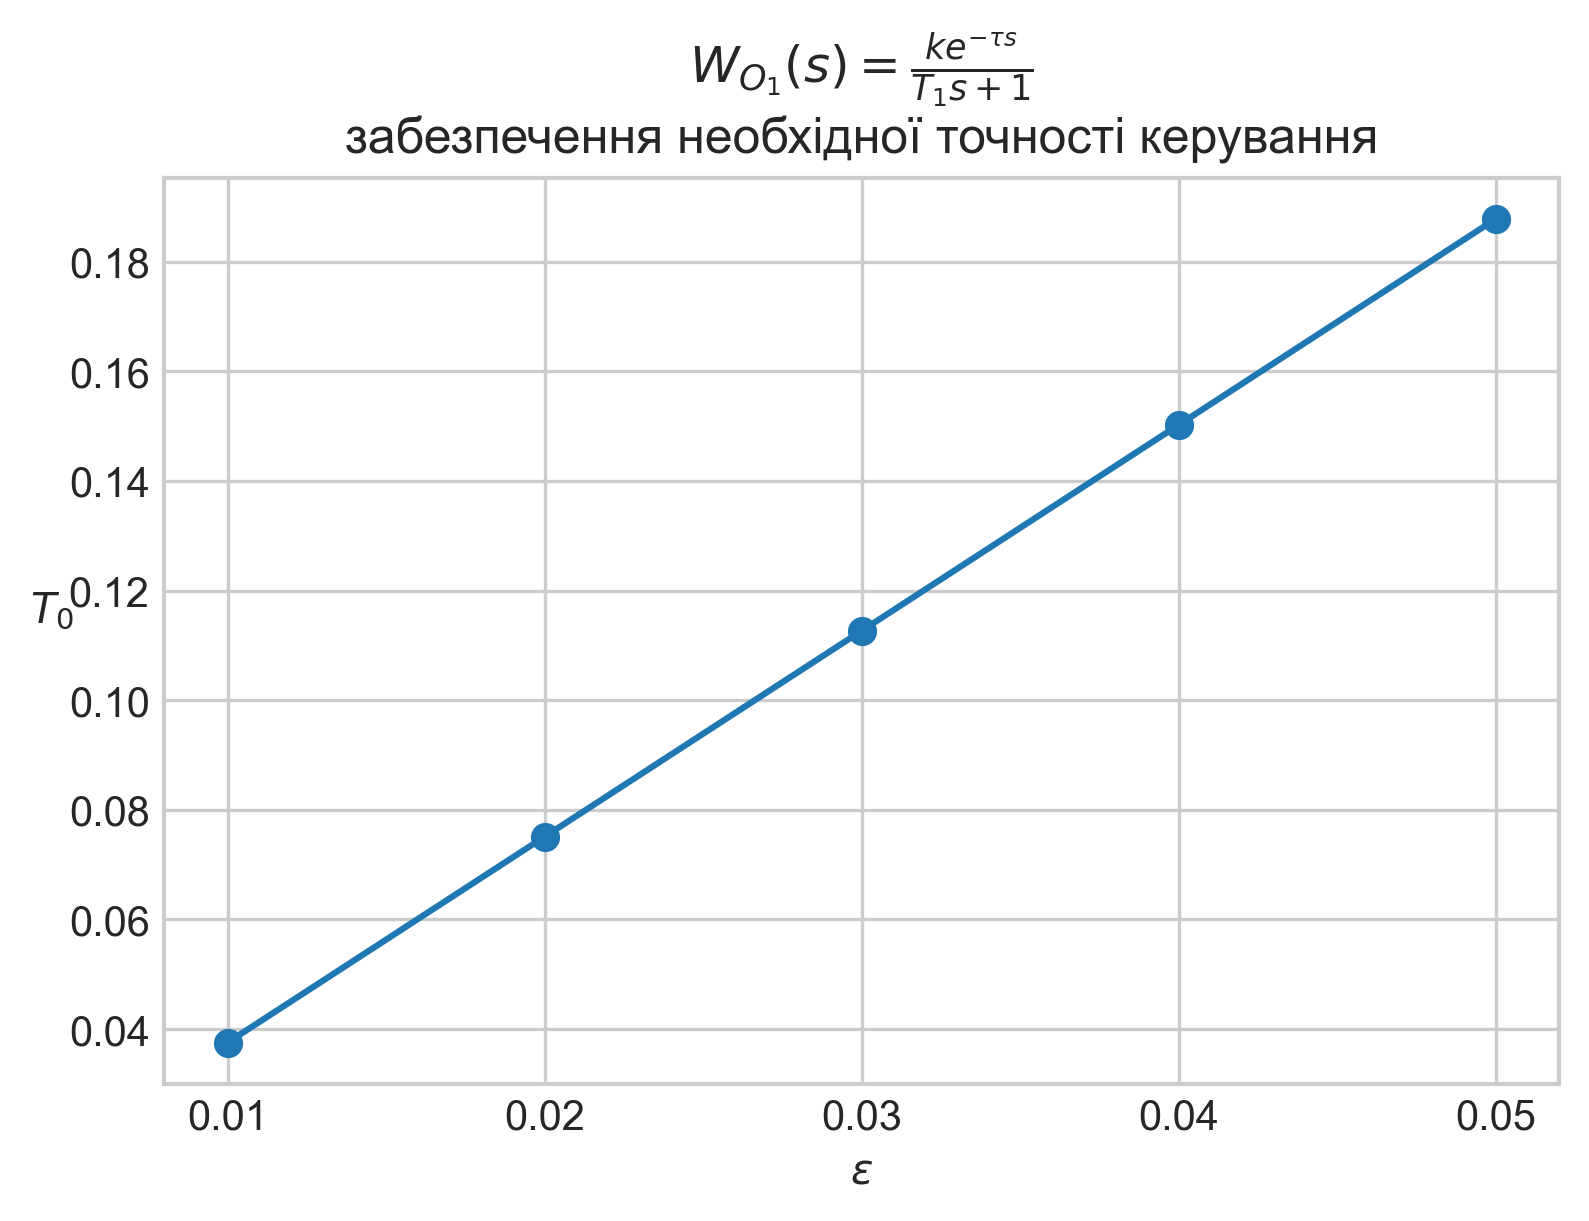
\includegraphics[scale=0.9]{pics/W_01_accur.png}
\end{center}
\subsection{Випадок \texorpdfstring{$W_{O_2}(s) = \frac{k e^{-\tau s}}{(T_1 s + 1)(T_2 s + 1)}$}{2}}
Знайдемо $B(\omega)$:
\begin{gather}
    \mbox{\normalsize $B(\omega) = \omega A(\omega) = \omega \cdot \left| W_{O_2}(j \omega)\right| = 
    \omega \cdot \frac{
        k \left| e^{-\tau j \omega}\right|
    }{
        \left|T_1 j \omega + 1\right| \left|T_2 j \omega + 1\right|
    } = \frac{k \omega}{\sqrt{\left(1 + T_1^2 \omega^2\right)\left(1 + T_2^2 \omega^2\right)}}$}
\end{gather}
$B_{\max}$ можна знайти за допомогою відповідної таблиці:
\begin{gather}
    B_{\max} = \frac{k}{T_1 + T_2} \Rightarrow T_0 = \frac{\varepsilon (T_1 + T_2)}{k}
\end{gather}
Отже, отримуємо наступні періоди квантування для різних $\varepsilon$:
\begin{center}
    \begin{tabular}{|c|c|c|c|c|c|}
        \hline
        $\varepsilon$ & $0.01$ & $0.02$ & $0.03$ & $0.04$ & $0.05$ \\
        \hline
        $T_0$ & $0.0579$ & $0.1159$ & $0.1738$ & $0.2318$ & $0.2897$ \\
        \hline
    \end{tabular}
\end{center}
Залежність $T_0$ від $\varepsilon$:
\begin{center}
    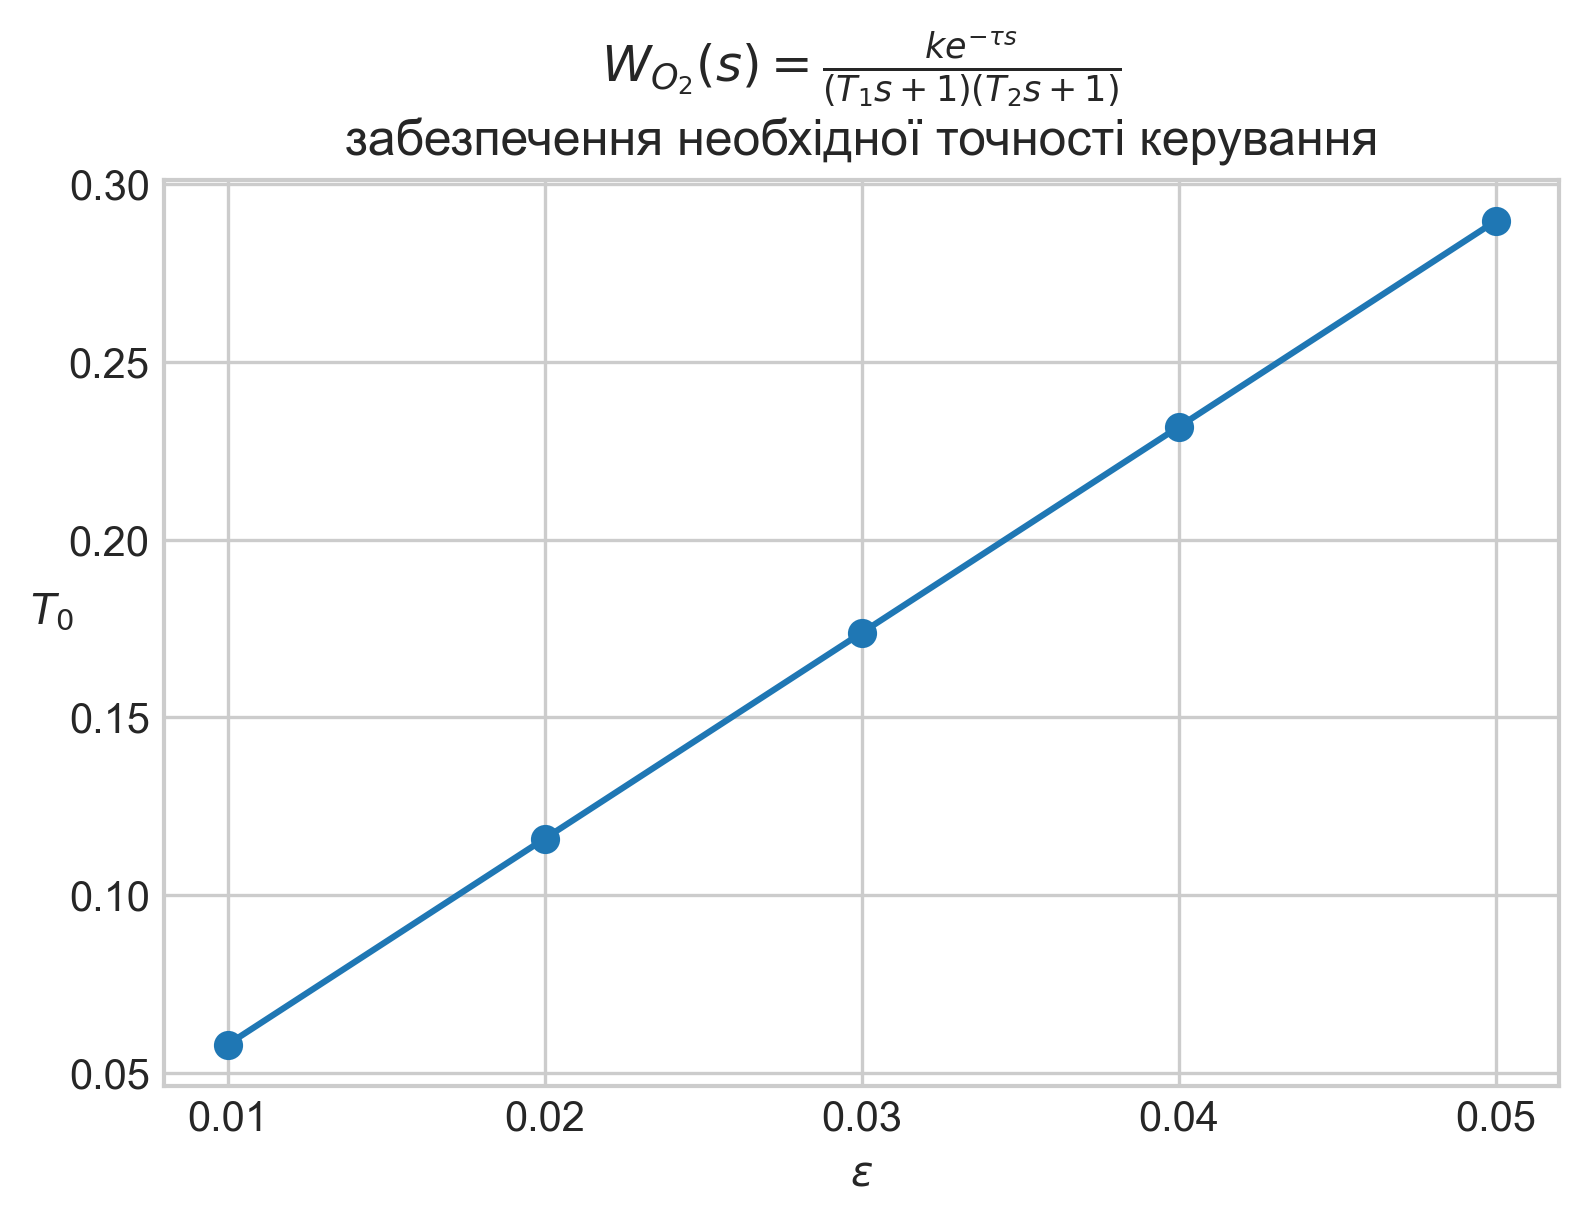
\includegraphics[scale=0.9]{pics/W_02_accur.png}
\end{center}
\section{Розрахунок за критерієм Джурі}
За цим критерієм період квантування обчислюється як $T_0 = \frac{\pi}{\omega_k}$, де 
$\omega_k$ -- розв'язок рівняння
\begin{gather}
    W_{\text{з}}(\omega_k) 
    = \left|
        \frac{W_O (j \omega_k) W_p (j \omega_k)}{
            1 + W_O (j \omega_k) W_p (j \omega_k)
        }
    \right| = \varepsilon
\end{gather}
$W_p =$ ???
\section{Розрахунок для об'єкта з динамікою в чисельнику}
Розглядається об'єкт з передаточною функцією $W_O(s) = \frac{
    k (T_1 s + 1)
}{
    (T_2 s + 1) (T_3 s + 1)
}$. Через те, що передаточна функція має динаміку в чисельнику, критерій забезпечення необхідної точності керування
та критерій Джурі непридатні для застосування. Приведемо передаточну функцію до вигляду
$W_O(s) = \frac{K (b T s + 1)}{T^2 s^2 + 2 \nu T s + 1}$:
\begin{gather*}
    \frac{
        k (T_1 s + 1)
    }{
        (T_2 s + 1) (T_3 s + 1)
    } = \frac{k (T_1 s + 1)}{T_2 T_3 s^2 + (T_2 + T_3) s + 1}
\end{gather*}
тому $T = \sqrt{T_2 T_3} \approx 14.4568$, $b = \frac{T_1}{T} \approx 2.421$, $\nu = \frac{T_2 + T_3}{2\sqrt{T_2 T_3}} = \frac{T_2 + T_3}{2T} \approx 1.0376$.
Знайдемо $\left|W_O (j \omega)\right|$:
\begin{gather*}
    \left|W_O (j \omega)\right| = \frac{
        k \left| bT \cdot j \omega + 1 \right|
    }{
        \left| -T^2 \omega^2 + 2\nu T \cdot j \omega + 1\right|
    } = 
    \frac{
        k \sqrt{1 + b^2 T^2 \omega^2}
    }{
        \sqrt{
            \left(1 - T^2 \omega^2\right)^2 + 4 \nu^2 T^2 \omega^2
        }
    }
\end{gather*}
Введемо $\omega_{\text{зр}} = \frac{q}{T}$ -- найвищу частоту сигналу, який необхідно відновити на виході системи:
\begin{gather*}
    \left|W_O (j \omega_{\text{зр}})\right| = 
    \frac{k\sqrt{1 + b^2 q^2}}{
        \sqrt{
            \left(1 - q^2\right)^2 + 4 \nu^2 q^2
        }
    }
\end{gather*}
Розв'яжемо рівняння $\left|W_O (j \omega_{\text{зр}})\right| = \frac{1}{\theta}$, де $\theta = 31$, відносно $q$:
\begin{gather*}
    \frac{k\sqrt{1 + b^2 q^2}}{
        \sqrt{
            \left(1 - q^2\right)^2 + 4 \nu^2 q^2
        }
    } = \frac{1}{\theta} \Leftrightarrow
    \frac{1 + b^2 q^2}{1 - 2 q^2 + q^4 + 4 \nu^2 q^2} = \frac{1}{k^2 \theta^2} \Leftrightarrow \\
    \Leftrightarrow 
    1 - 2 q^2 + q^4 + 4 \nu^2 q^2 = k^2 \theta^2 \left(1 + b^2 q^2\right) \Leftrightarrow \\
    \Leftrightarrow
    q^4 + q^2 \left(4 \nu^2 - b^2 k^2 \theta^2 - 2\right) q^2 + \left(1 - k^2 \theta^2\right) = 0
\end{gather*}
Розв'яжемо це рівняння спочатку відносно $q^2$. Приблизні значення коренів: 
\begin{gather*}
    \left[
        \begin{array}{ll}
            q^2 = 489261.8397 \\
            q^2 = -0.17061
        \end{array}
    \right.
\end{gather*}
Оскільки комплексні та від'ємні $q$ не розглядаються, то отримуємо $q \approx 699.4725$.
Отже, період квантування $T_0 = \frac{\pi}{\omega_{\text{зр}}} = 
\frac{\pi T}{q} = 0.0649$.